% Options for packages loaded elsewhere
\PassOptionsToPackage{unicode}{hyperref}
\PassOptionsToPackage{hyphens}{url}
%
\documentclass[
]{article}
\usepackage{lmodern}
\usepackage{amssymb,amsmath}
\usepackage{ifxetex,ifluatex}
\ifnum 0\ifxetex 1\fi\ifluatex 1\fi=0 % if pdftex
  \usepackage[T1]{fontenc}
  \usepackage[utf8]{inputenc}
  \usepackage{textcomp} % provide euro and other symbols
\else % if luatex or xetex
  \usepackage{unicode-math}
  \defaultfontfeatures{Scale=MatchLowercase}
  \defaultfontfeatures[\rmfamily]{Ligatures=TeX,Scale=1}
\fi
% Use upquote if available, for straight quotes in verbatim environments
\IfFileExists{upquote.sty}{\usepackage{upquote}}{}
\IfFileExists{microtype.sty}{% use microtype if available
  \usepackage[]{microtype}
  \UseMicrotypeSet[protrusion]{basicmath} % disable protrusion for tt fonts
}{}
\makeatletter
\@ifundefined{KOMAClassName}{% if non-KOMA class
  \IfFileExists{parskip.sty}{%
    \usepackage{parskip}
  }{% else
    \setlength{\parindent}{0pt}
    \setlength{\parskip}{6pt plus 2pt minus 1pt}}
}{% if KOMA class
  \KOMAoptions{parskip=half}}
\makeatother
\usepackage{xcolor}
\IfFileExists{xurl.sty}{\usepackage{xurl}}{} % add URL line breaks if available
\IfFileExists{bookmark.sty}{\usepackage{bookmark}}{\usepackage{hyperref}}
\hypersetup{
  hidelinks,
  pdfcreator={LaTeX via pandoc}}
\urlstyle{same} % disable monospaced font for URLs
\usepackage[margin=1in]{geometry}
\usepackage{longtable,booktabs}
% Correct order of tables after \paragraph or \subparagraph
\usepackage{etoolbox}
\makeatletter
\patchcmd\longtable{\par}{\if@noskipsec\mbox{}\fi\par}{}{}
\makeatother
% Allow footnotes in longtable head/foot
\IfFileExists{footnotehyper.sty}{\usepackage{footnotehyper}}{\usepackage{footnote}}
\makesavenoteenv{longtable}
\usepackage{graphicx}
\makeatletter
\def\maxwidth{\ifdim\Gin@nat@width>\linewidth\linewidth\else\Gin@nat@width\fi}
\def\maxheight{\ifdim\Gin@nat@height>\textheight\textheight\else\Gin@nat@height\fi}
\makeatother
% Scale images if necessary, so that they will not overflow the page
% margins by default, and it is still possible to overwrite the defaults
% using explicit options in \includegraphics[width, height, ...]{}
\setkeys{Gin}{width=\maxwidth,height=\maxheight,keepaspectratio}
% Set default figure placement to htbp
\makeatletter
\def\fps@figure{htbp}
\makeatother
\setlength{\emergencystretch}{3em} % prevent overfull lines
\providecommand{\tightlist}{%
  \setlength{\itemsep}{0pt}\setlength{\parskip}{0pt}}
\setcounter{secnumdepth}{5}

\author{}
\date{\vspace{-2.5em}}

\begin{document}

\renewcommand{\figurename}{Supplementary Figure}
\pagenumbering{gobble}

\newpage

\begin{figure}
\centering
\includegraphics{suppl_figs/suppl_fig3.pdf}
\caption{\label{fig:sup-fig-3}\textbf{Random sampling of k-NN graph vertices is suboptimal compared to sampling with refinement.}
(A) Sampling with refinement leads to selection of fewer neighbourhoods
(B) Sampling with refinement leads to selection of bigger neighbourhoods for DA testing, independently of the initial proportion of cells sampled
(C) Sampling with refinement generates robust neighbourhoods across initializations: for each index cell we calculate the distance from the closest index in a sampling with different initialization. The cumulative distribution of distances to the closest index is shown. The black dotted line denotes the distribution of distances between k nearest neighbors in the dataset (k=30) (NH: neighbourhood).
Neighbourhood statistics were calculated using a simulated trajectory dataset of 5000 cells. All plots show results from three sampling initializations for each proportion.}
\end{figure}







\begin{figure}
\centering
\includegraphics{suppl_figs/suppl_fig1.pdf}
\caption{\label{fig:sup-fig-1}\textbf{Tolerance of Milo to uncorrected batch effects in simulated data}
(A-B) UMAP embeddings of simulated scRNA-seq data containing a batch effect, before batch correction (top row) and after correction with fastMNN (bottom row) (5000 cells). Cells are colored by simulated batch (A) and by presence of differential abundance between 2 simulated conditions (20\% cells in condition `A', 80\% cells in condition `B') (B).
(C) A graph representation of the results from Milo differential abundance testing. Neighbourhoods were tested for DA between conditions, with (\textasciitilde{} batch + condition) or without (\textasciitilde{} condition) accounting for the simulated batch. Nodes are neighbourhoods, coloured by their log fold change between conditions. Non-DA neighbourhoods (FDR 10\%). Node sizes correspond to the number of cells in a neighbourhood. Graph edges depict the number of cells shared between adjacent neighbourhoods.
(D) Confusion matrices comparing the number of true and predicted DA neighbourhoods, with different batch effect correction (rows) and different testing design (columns).}
\end{figure}






\begin{figure}
\centering
\includegraphics{suppl_figs/suppl_fig2.pdf}
\caption{\label{fig:sup-fig-2}\textbf{Tolerance of Milo to uncorrected batch effects in mouse gastrulation atlas}
(A-B) UMAP embedding of mouse gastrulation atlas before batch correction (top row) and after correction with fastMNN (bottom row). Cells are colored by sequencing batch (A) and developmental time point (B).
(C) Barplot depicting the percentage of DA neighbourhoods at FDR 10\%, testing for different experimental covariates: DA between sequencing batches (\textasciitilde{} Seq. batch), DA across developmental time points (\textasciitilde{} Time points), DA across developmental time points accounting for the sequencing batch (\textasciitilde{} Seq. batch + time points). The total number of DA neighbourhoods is shown in each bar.}
\end{figure}





\begin{figure}
\centering
\includegraphics{suppl_figs/suppl_fig4.pdf}
\caption{\label{fig:sup-fig-4}\textbf{Graph-clustering does not faithfully capture simulated groups and differentially abundant subpopulations in a simulated continuous trajectory.}
(A) A simulated linear trajectory of 2000 single-cells generated from 5 different groups, with cells assigned to either condition `A' (left) or condition `B' (right).
(B) A Walktrap clustering of the data in (A) using the same k-NN graph. Cells are coloured by Walktrap cluster identity.
(C) A Louvain clustering of the data in (A) using the same k-NN graph. Cells are coloured by the Louvain clustering identity.
(D-E) Heatmaps comparing the numbers of cells in each cluster with respect to the ground truth groups in (A). Each cell is coloured by the proportion of cells from the column groups (ground truth) that are assigned to the respective cluster.}
\end{figure}







\begin{figure}
\centering
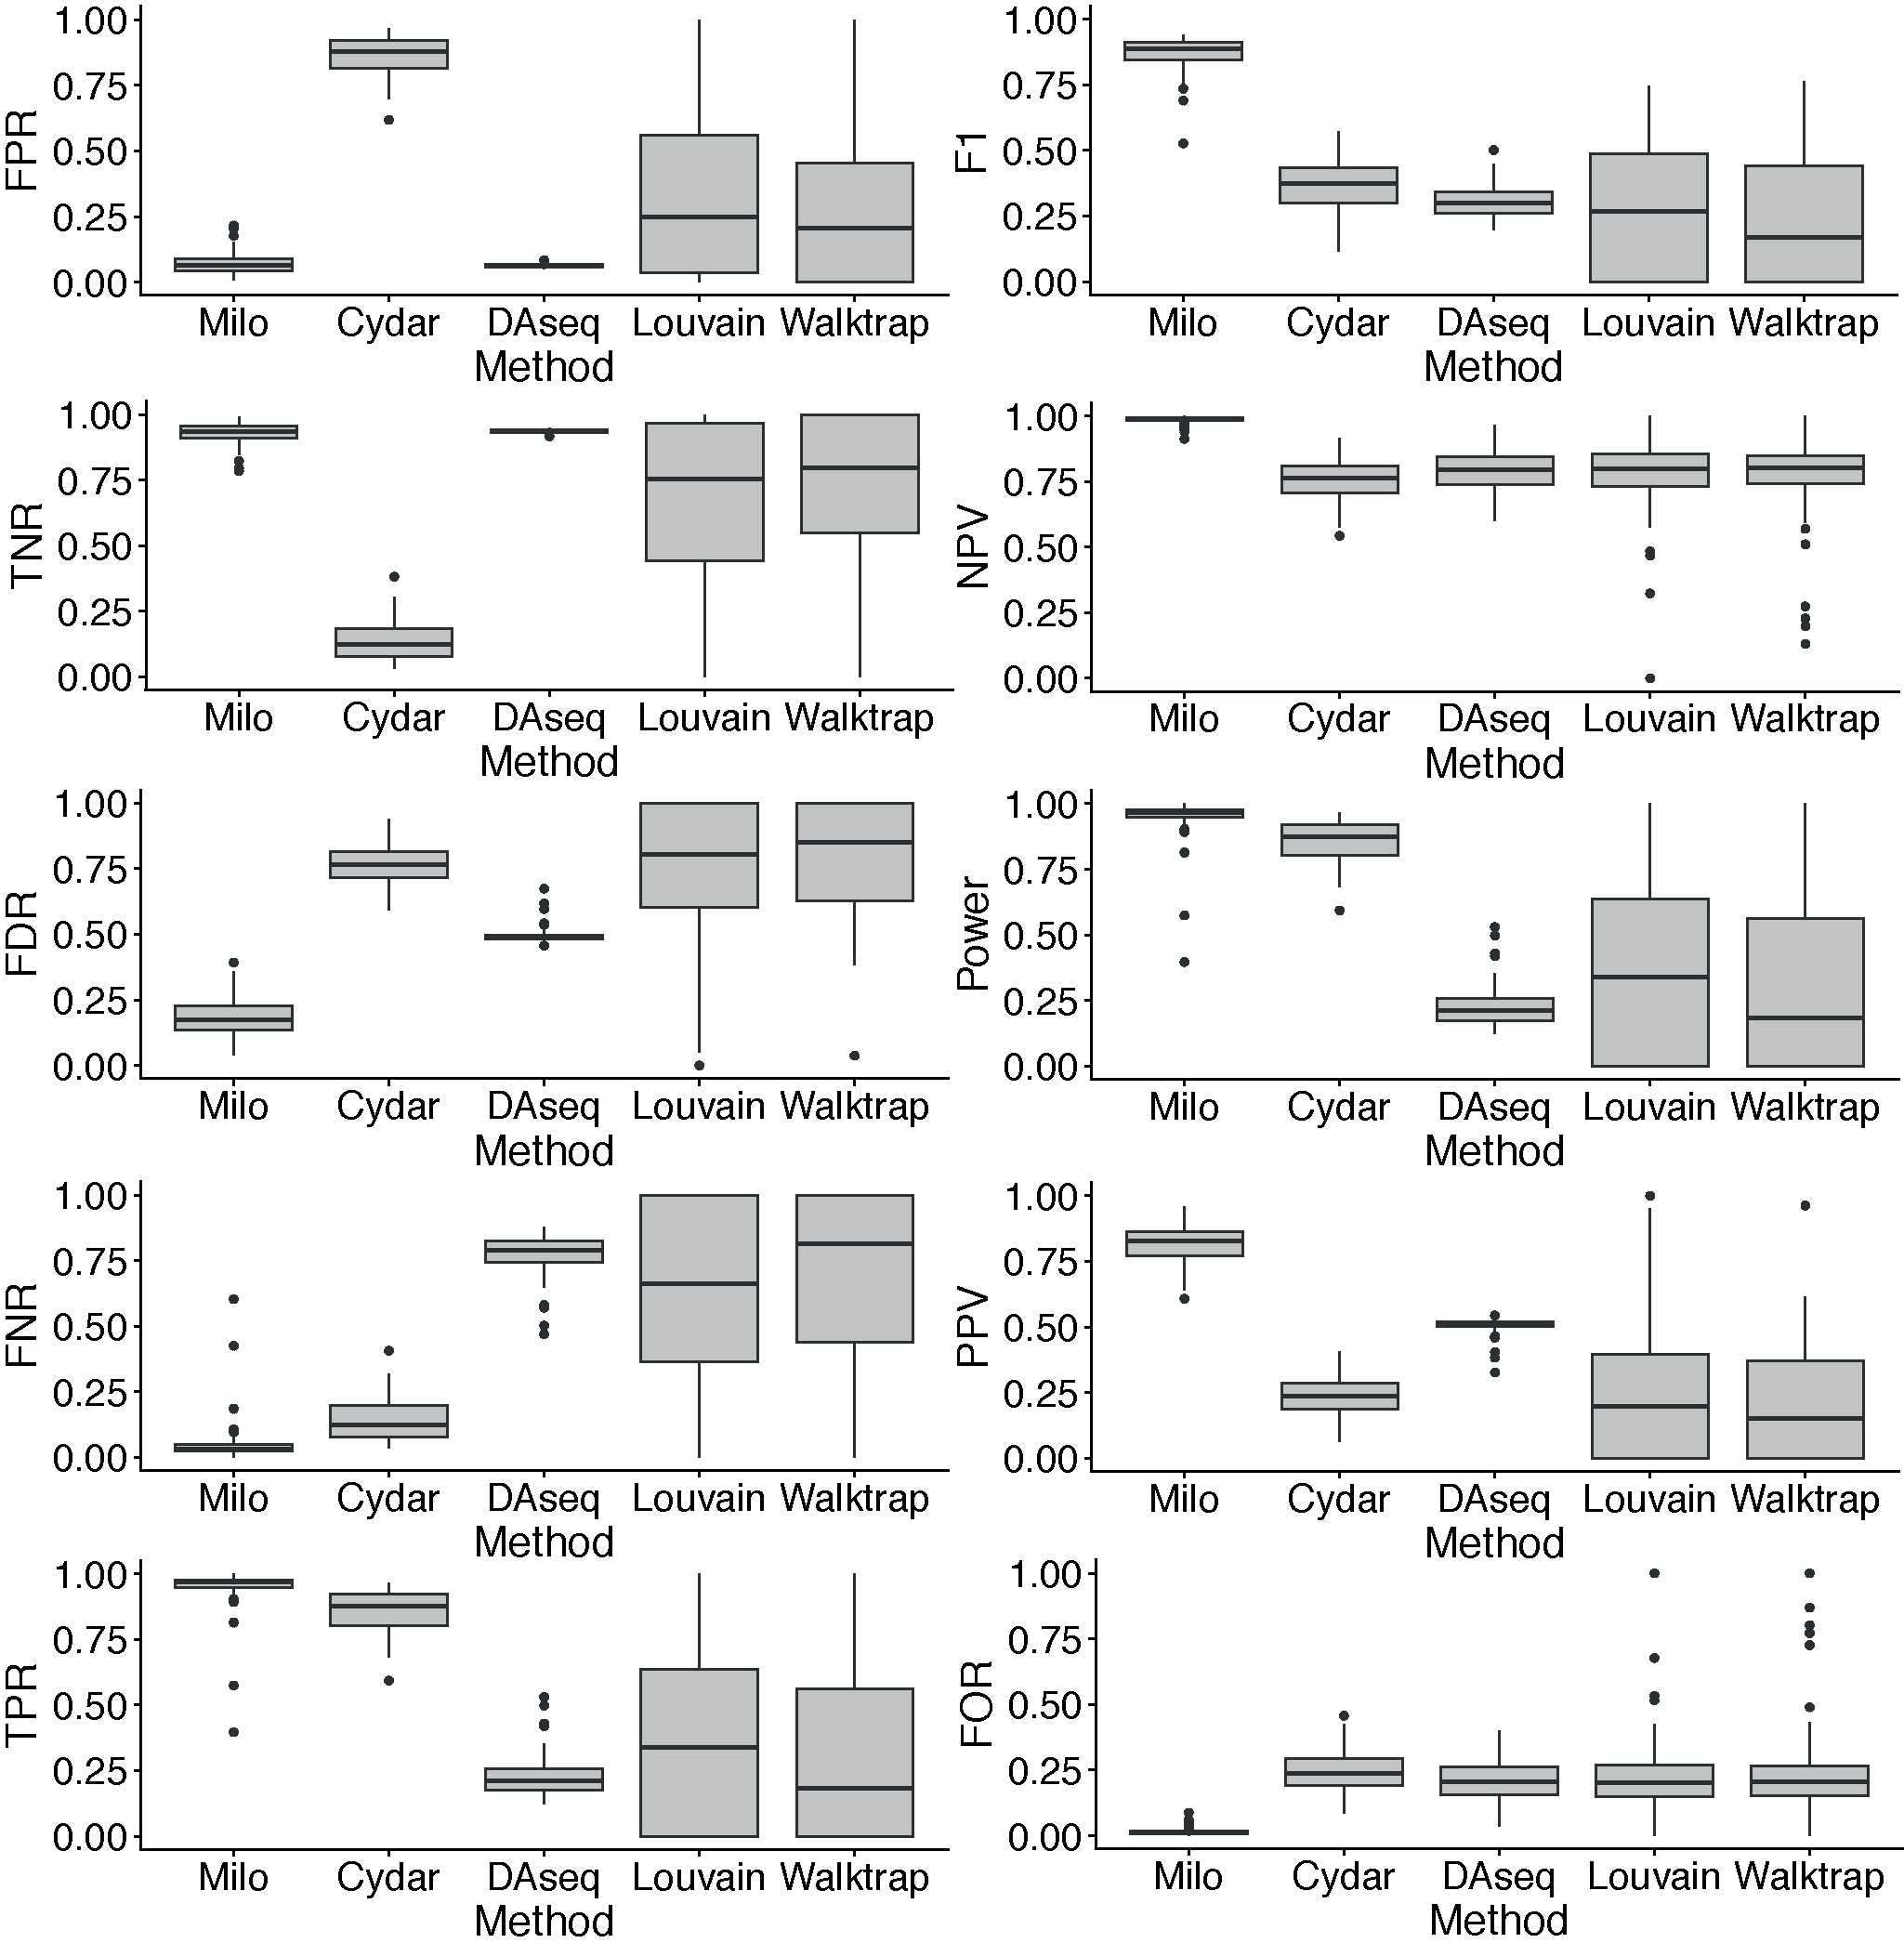
\includegraphics{suppl_figs/suppl_fig5.pdf}
\caption{\label{fig:sup-fig-5}\textbf{Comparison of Milo to alternative differential abundance methods}
Each panel shows a measure of method performance computed across 100 independent simulations. Boxplots denote the median and interquartile range (IQR), with whiskers extending 1.5 x IQR; outliers are shown as individual points. Each analysis on each independent simulation used the same parameter values in Supplementary Table 1.}
\end{figure}




\begin{figure}
\centering
\includegraphics{suppl_figs/suppl_fig7.pdf}
\caption{\label{fig:sup-fig-7}\textbf{Memory usage across the Milo analysis workflow}
Total memory usage across the steps of the Milo analysis workflow in 4 data sets containing different numbers of cells (Gastrulation: circles, Liver: triangles, Thymus: crosses, Simulation: squares). Grey points denoted down-sampled datasets of the corresponding type. Coloured points denote the total number of cells for the respective dataset. Total memory usage (y-axis) is shown in megabytes (MB). (A) k-NN graph building, (B) neighbourhood sampling and construction, (C) within-neighbourhood distance calculation, (D) cell counting in neighbourhoods according to the input experimental design, (E) differential abundance testing, (F) total in memory R object size. A fixed value was used in all data-sets for graph building and neighbourhood construction (k=30).}
\end{figure}




\begin{figure}
\centering
\includegraphics{suppl_figs/suppl_fig6.pdf}
\caption{\label{fig:sup-fig-6}\textbf{Downstream analysis of disease-specific subpopulations in liver cirrhosis}
(A) GO term enrichment analysis on marker genes of cirrhosis-enriched endothelia. The top 20 significant terms are shown.
(B) GO term enrichment analysis on marker genes of healthy-enriched endothelia. The top 20 significant terms are shown.
(C) UMAP embedding and graph representation of neighbourhoods of 3369 cells from cholangiocytes lineage.
(D) Volcano plot for DGE test on cholangiocytes DA subpopulations: the x-axis shows the log-fold change between expression in cirrhotic and healthy cholangiocytes. The y-axis shows the adjusted p-value.
(E) GO term enrichment analysis on marker genes of cirrhosis-enriched cholangiocytes. The top 20 significant terms are shown.}
\end{figure}








\newpage

\hypertarget{supplementary-tables}{%
\section{Supplementary tables}\label{supplementary-tables}}

\begin{longtable}[]{@{}llll@{}}
\toprule
Method & Key Parameters & Values & Hypothesis testing\tabularnewline
\midrule
\endhead
Milo & K & 10 & Negative binomial GLM, 10\% FDR\tabularnewline
& d & 15 & Negative binomial GLM, 10\% FDR\tabularnewline
Cydar & r & 2 & Negative binomial GLM, 10\% FDR\tabularnewline
DAseq & k.vector & 5-500, steps of 50 & Logistic classifier prediction, top 10\%\tabularnewline
Louvain + edgeR & K & 10 & Negative binomial GLM, 10\% FDR\tabularnewline
& d & 15 &\tabularnewline
Walktrap + edgeR & K & 10 & Negative binomial GLM, 10\% FDR\tabularnewline
& d & 15 &\tabularnewline
\bottomrule
\end{longtable}

Supplementary Table 1: \textbf{Method comparison parameter values.}

\newpage

\end{document}
